\section{Verificatie}

%inleiding over welke testen we gaan uitvoeren en waarom. Over hoe de testen zijn opgesteld en wat het doel is van de totaliteit testen.

\subsection{Enkele communicatie Test}
% uitleg wat de test is met doel
Deze test kijkt naar de communicatie tussen twee nodes. Het doel is om te kijken hoe betrouwbaar de connectie is en 
over welke afstand de communicatie nog steeds betrouwbaar is. De test zal beginnen door eerst 100 berichten naar de andere 
node te sturen op een afstand van 10 cm en te kijken hoeveel van de berichten aankomt bij de andere node. Zo zal na elke test de 
afstand worden vergroot totdat de betrouwbaarheid onder de 90\% komt. Daarna is de kans dat een bericht voor onze specificaties te 
klein en op deze manier weten we ook meteen hoever de nodes van elkaar af moeten staan. De betrouwbaarheid wordt gebasseerd op de 
hoeveelheid aan berichten dat is aangekomen van de 100 berichten. Daarnaast wordt ook de trust levels vastgelegd 
die het systeem zelf meet. Dit wordt gedaan om de data met elkaar te vergelijken en hier conclusies aan vast te leggen.
% Test opstelling
In onderstaande afbeelding \ref{fig:TestCom} is de testopstelling opgezet. Te zien is dat er twee xmega's nodig zijn met een NRF chip. 
Deze moeten naar elkaar kijken en worden na elke test met afstand vergroot. Bij deze test zal er niks tussen de verbinding zitten.
\begin{figure}[h]
    \centering
    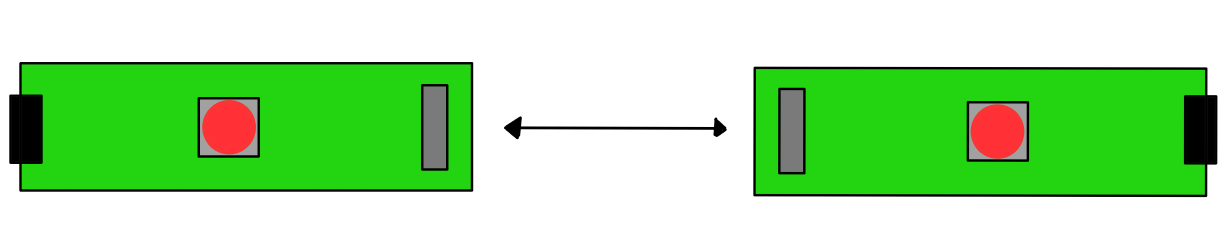
\includegraphics{img/Screenshot_292.png}
    \caption{Test opstelling}
    \label{fig:TestCom}
\end{figure}
% Resultaten test
In onderstaande tabel \ref{Test:EnkelCom} zijn de testresultaten te zien.
\begin{table}[h]
    \centering
    \begin{tabular}{|c||c|c|c|c|}
        \hline
        Test    & Afstand   & Aangekomen berichten  & Trust & Betrouwbaarheid   \\\hline\hline
        Test 1  & 10 cm     &                       &       &                   \\\hline
        Test 2  & 15 cm     &                       &       &                   \\\hline
        Test 3  & 20 cm     &                       &       &                   \\\hline
        Test 4  & 30 cm     &                       &       &                   \\\hline
        Test 5  & 50 cm     &                       &       &                   \\\hline
        Test 6  & 100 cm    &                       &       &                   \\\hline
        Test 7  & 150 cm    &                       &       &                   \\\hline
        Test 8  & 200 cm    &                       &       &                   \\\hline   
    \end{tabular}
    \caption{Testresultaten Enkele communicatie Test}
    \label{Test:EnkelCom}
\end{table}

\subsection{Hop Test}
% uitleg wat de test is met doel
Deze test is vergelijkbaar met vorige test, maar maakt gebruik van één extra node tussen de twee versturende en ontvangende nodes. 
Het doel van deze test is om te kijken hoe betrouwbaar de hop communicatie is. Ook kan er gekeken worden op welke maximale afstand 
de hops ook nog steeds werken. 
% Test opstelling
Voor deze test zijn drie nodes nodig. In onderstaande afbeelding \ref{fig:Testhop} is te zien hoe de nodes moeten staan.
 Één die ontvangt, één die verstuurd en één die gebruikt wordt als hop. Ook voor deze test wordt er na elke test 
 de afstand tussen de nodes vergroot. Dit wordt per kant gedaan. Dus eerst vergroot de rechterkant met een kleine afstand 
en dan vergroot de linkerkant van de hop node tussen de andere node met een kleine afstand.

\begin{figure}[h]
    \centering
    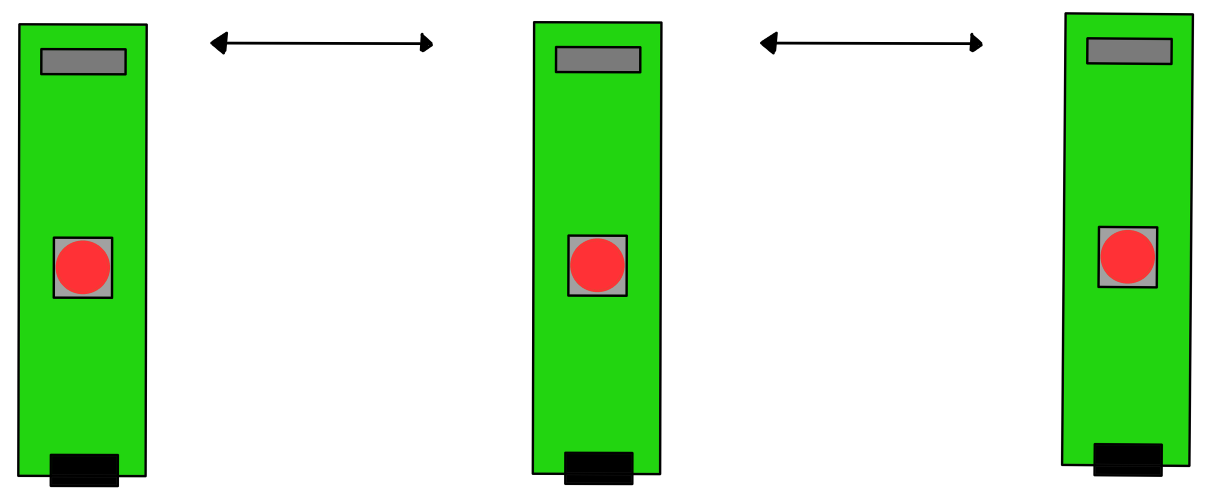
\includegraphics{img/Screenshot_293.png}
    \caption{Test opstelling 2}
    \label{fig:Testhop}
\end{figure}

% Resultaten test
\begin{table}[h]
    \centering
    \begin{tabular}{|c||c|c|c|c|}
        \hline
        Test    & Afstand rechterkant  & Afstand linkerkant & Aangekomen berichten  & Trust & Betrouwbaarheid   \\\hline\hline
        Test 1  & 10 cm                & 10 cm              &                       &       &                   \\\hline
        Test 2  & 15 cm                & 10 cm              &                       &       &                   \\\hline
        Test 3  & 15 cm                & 15 cm              &                       &       &                   \\\hline
        Test 4  & 30 cm                & 15 cm              &                       &       &                   \\\hline
        Test 5  & 30 cm                & 30 cm              &                       &       &                   \\\hline
        Test 6  & 50 cm                & 30 cm              &                       &       &                   \\\hline
        Test 7  & 50 cm                & 50 cm              &                       &       &                   \\\hline
        Test 8  & 100 cm               & 50 cm              &                       &       &                   \\\hline
        Test 9  & 100 cm               & 100 cm             &                       &       &                   \\\hline 
        Test 10 & 200 cm               & 100 cm             &                       &       &                   \\\hline 
        Test 11 & 200 cm               & 200 cm             &                       &       &                   \\\hline   
    \end{tabular}
    \caption{Testresultaten Hop Test}
    \label{Test:Hop}
\end{table}

\subsection{Totale communicatie Test}
% uitleg wat de test is met doel
Het doel van deze test is een samenstelling van de vorige 2 testen. Deze test zal kijken naar de communicatie tussen meerdere nodes.
Elke node zal 100 berichten versturen naar een zelf uitgekozen node. Dit moet naar een node met 1 of meerdere hops en een directe node.
De afstand zal bij deze test statisch zijn. Het doel van deze test is om te zien of de communicatie met meerdere nodes lukt en om te zien 
of elke node een beetje dezelfde resulaten toont. 
% Test opstelling
Omdat de opdracht van dit verslag kijkt naar vijf sensoren met een basisstation zal voor deze test 6 afzonderlijke nodes gebruikt worden.
In onderstaande afbeelding \ref{fig:TestTotCom} is te zien hoe de xmega's opgesteld moeten worden. De afstand is gebasseerd op de grootst 
mogelijke afstand waarbij de betrouwbaarheid nog boven de 90\% ligt vanuit de enkele communicatie test.

\begin{figure}[h]
    \centering
    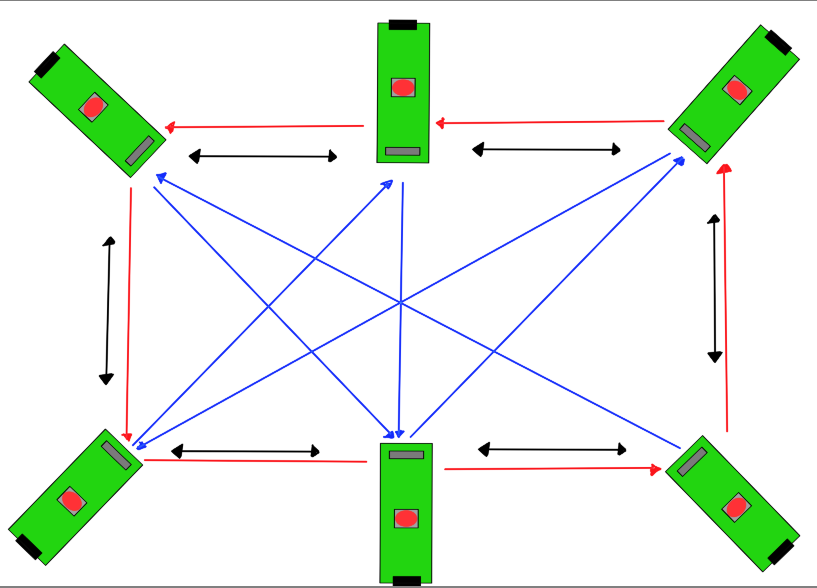
\includegraphics{img/Screenshot_294.png}
    \caption{Test opstelling 3}
    \label{fig:TestTotCom}
\end{figure}
% Resultaten test
In onderstaande tabel \ref{Test:TotCom} zijn de test resulaten te zien. Zowel de directe buur restulaten als de Indirecte buur resultaten staan 
in hetzelfde tabel.
\begin{table}[h]
    \centering
    \begin{tabular}{|c||c|c|c|c|c|c|}
        \hline
        \textbf{Test}    & \textbf{Node}  & \textbf{Directe buur}   & \textbf{Aangekomen berichten}  & \textbf{Trust}     & \textbf{Betrouwbaarheid}   &\\\hline\hline
        Test 1  &       &                &                       &           &                   &\\\hline
        Test 2  &       &                &                       &           &                   &\\\hline
        Test 3  &       &                &                       &           &                   &\\\hline
        Test 4  &       &                &                       &           &                   &\\\hline
        Test 5  &       &                &                       &           &                   &\\\hline
        Test 6  &       &                &                       &           &                   &\\\hline\hline
        \textbf{Test}    & \textbf{Node}  & \textbf{Indirecte buur}   & \textbf{Aantal hops} \textbf{Aangekomen berichten}  & \textbf{Trust}     & \textbf{Betrouwbaarheid}   \\\hline\hline
        Test 1  &       &                &           &            &           &                   \\\hline
        Test 2  &       &                &           &            &           &                   \\\hline
        Test 3  &       &                &           &            &           &                   \\\hline
        Test 4  &       &                &           &            &           &                   \\\hline
        Test 5  &       &                &           &            &           &                   \\\hline
        Test 6  &       &                &           &            &           &                   \\\hline\hline
    \end{tabular}
    \caption{Testresultaten Totale communicatie Test}
    \label{Test:TotCom}
\end{table}

\subsection{Encryptie Test}
% uitleg wat de test is met doel
Deze test kijkt of de encryoptie goed is geimplementeerd. Dit wordt gedaan door 2 nodes te pakken en bij 1 node de encryptie uit te zetten.
dan wordt er gekeken naar wat binnen komt en wordt met de hand dit bericht omcijferd. Nadat dat is gedaan wordt de encryptie weer aangezet 
om te kijken of dit overeenkomt met wat is verstuurd. Het doel van deze test is om de betrouwbaarheid van de encryptie te bekijken.
% Test opstelling
De opstelling is hetzelfde zoals de enkele communicatie test. Het enige verschil is de encryptie die bij 1 node aan staat en bij de andere uit.
\begin{figure}[h]
    \centering
    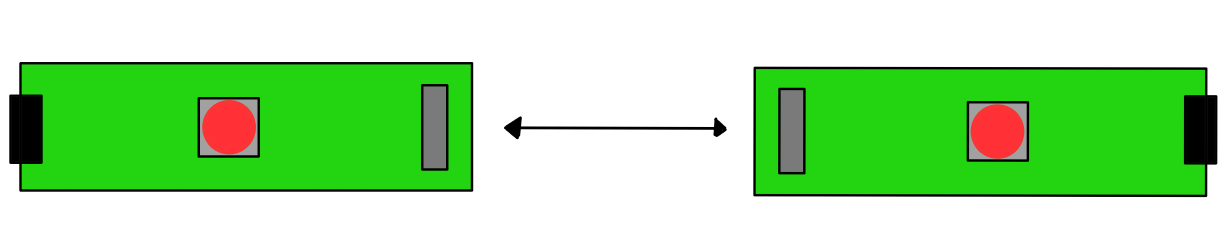
\includegraphics{img/Screenshot_292.png}
    \caption{Test opstelling}
    \label{fig:TestCom}
\end{figure}
% Resultaten test
\begin{table}[h]
    \centering
    \begin{tabular}{|c||c|c|c|c|c|c|}
        Test    & Verzonden bericht      & Key 1 & Key 2 & Ontvangen bericht & Zelf Decrypted bericht & Decrypted bericht \\\hline
        Test 1  & Hallo                  &       &       &                   &                        &                   \\\hline
        Test 2  & Poezen zijn lief       &       &       &                   &                        &                   \\\hline
        Test 3  & Opdracht 1 met ?       &       &       &                   &                        &                   \\\hline
        Test 4  & is deze opdracht leuk? &       &       &                   &                        &                   \\\hline
    \end{tabular}
    \caption{Testresultaten Totale communicatie Test}
    \label{Test:TotCom}
\end{table}

\subsection{Interface Test}
% uitleg wat de test is met doel
Deze test kijkt naar de interface van het basis station. Het scherm bevat, zoals eerder gelezen, een debug scherm en een gebruikers scherm. 
In beide gevallen wil je zeker weten dat beide schermen werken zoals verwacht. Deze test zal dit dan ook testen. Er zullen voor de 
interface test 2 testen uitgevoerd worden. Één voor het debug scherm en één voor het gebruikers scherm.

\subsubsection{Debug scherm}
% Test opstelling
Voor deze test zijn vijf nodes nodig en het basisstation. Het basisstation zal 100 keer naar elke node een Ping of Life sturen en elke node zal 
naar het basisstation 100 berichten versturen. Op het basisstation zal ook bekeken worden hoe groot de trust is van elke node voor de Ping of Life.

% Resultaten test
\begin{table}[h]
    \centering
    \begin{tabular}{|c||c|c|c|c|}
        \textbf{Test}   &   \textbf{Ontvangen door} & \textbf{Aangekomen berichten} &   \textbf{Trust}  &   \textbf{Betrouwbaarheid}    \\\hline
        Test 1          &                           &                               &                   &                               \\\hline 
        Test 2          &                           &                               &                   &                               \\\hline 
        Test 3          &                           &                               &                   &                               \\\hline 
        Test 4          &                           &                               &                   &                               \\\hline 
        Test 5          &                           &                               &                   &                               \\\hline 
        \textbf{Test}   &   \textbf{Verzonden naar} & \textbf{Aangekomen berichten} &   \textbf{Trust}  &   \textbf{Betrouwbaarheid}    \\\hline
        Test 1          &                           &                               &                   &                               \\\hline 
        Test 2          &                           &                               &                   &                               \\\hline 
        Test 3          &                           &                               &                   &                               \\\hline 
        Test 4          &                           &                               &                   &                               \\\hline 
        Test 5          &                           &                               &                   &                               \\\hline 
    \end{tabular}
    \caption{Testresultaten Interface Test}
    \label{Test:Int}
\end{table}

